\documentclass[10pt]{article}

\def\Type{LessonDJ}
\def\TypeNum{Workshop Week 11} %Lesson #
\def\TypeTitle{KC3 Review} %Lesson Title
\def\Semester{Fall 2021} %Not Used 
\def\Course{MATH 1190}%Course number and name
\def\Targets{ \target{I1}, \target{I2}, \target{A2} }

\usepackage{preambleDJ} 

%%%%%%%%%%%% BEGIN DOCUMENT %%%%%%%%%%%%%%%
%%%%%%%%%%%% BEGIN DOCUMENT %%%%%%%%%%%%%%%
%%%%%%%%%%%% BEGIN DOCUMENT %%%%%%%%%%%%%%%
%%%%%%%%%%%% BEGIN DOCUMENT %%%%%%%%%%%%%%%
%%%%%%%%%%%% BEGIN DOCUMENT %%%%%%%%%%%%%%%

\begin{document}
\pagestyle{otherpages}
\thispagestyle{firstpage}


\vs{.6}
\section{Definite Integrals}
\begin{enumerate}
    \item Consider the graph of $f(x) = -x^3+x+1$\\
    \mpageT{.4}{.6}{
       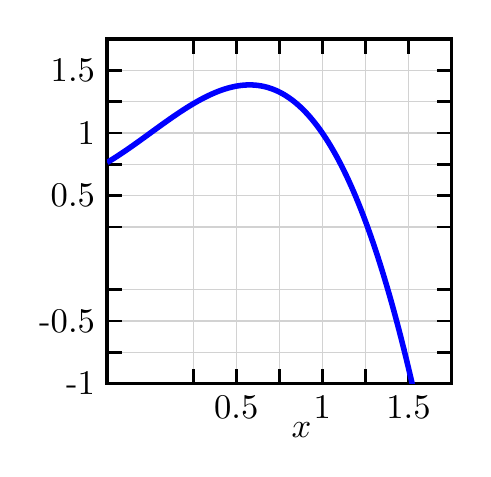
\begin{tikzpicture}[scale=1.25]
          \begin{axis}[
        %    axis y line = left,
            axis  line style= {line width = 1pt},
            xlabel={$x$},
            xtick       = {0.25,0.5,0.75,1,1.25,1.5,1.75},
            xticklabels = {,0.5,,1,,1.5},
            ytick       = {-1,-.75,-.5,-.25,0.25,0.5,0.75,1,1.25,1.5,1.75},
             yticklabels = {-1,,-0.5,,,0.5,,1,,1.5,},
             major tick style = {black, thick},
            xlabel style={anchor=west},
            ylabel style={anchor=south},
            samples     = 160,
            domain      = -.25:1.75,
            xmin = -0.25, xmax = 1.75,
            ymin = -1, ymax = 1.75,
            grid=both, grid style={gray!35},
            width=2in, height=2.in
          ]
          \addplot[domain=-0.25:1.75, blue, ultra thick, -] {-x^3+x+1};
        \end{axis}
    \end{tikzpicture}
    }{
%    \graphicsC{week11_spring.png}{3}
%    \begin{center}
%        
\includegraphics[scale = 0.5]{Fall 2025/1190 discussion/week11/images/week11_spring.png}
%    \end{center}
    \begin{enumerate}
        \item[(a)] Using $3$ boxes, approximate the definite integral $\ds \int_0^{1.5} f(x) dx.$ Note, that you certainly won't get the exact answer!
    \end{enumerate}
    }
    \enum{
            \item[(b)] If $f(x)$ is a function of velocity (in miles per hour) of a car on the highway (looks like he turned around and booked it!) and we know that at time $t=0$ that the car was at position $m =1000$ meters, what is the position of the car at time $1.5.$ Give your answer using a definite integral. 
            }
    \newpage
    \item Consider the function $f(x) = |x|.$\\
    \mpageT{.4}{.6}{
           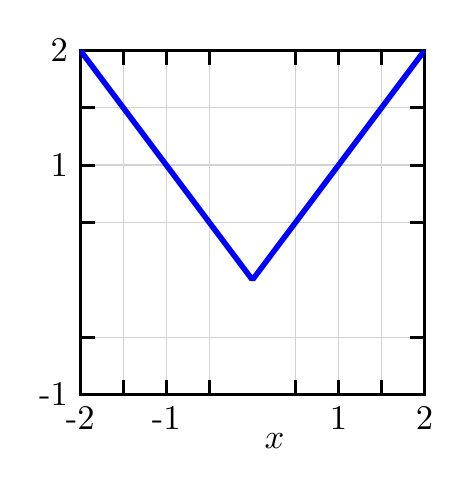
\begin{tikzpicture}[scale=1.25]
          \begin{axis}[
        %    axis y line = left,
            axis  line style= {line width = 1pt},
            xlabel={$x$},
            xtick       = {-2,-1.5,-1,-.5, .5,1,1.5,2},
            xticklabels = {-2,,-1,,,1,,2},
            ytick       = {-1,-.5,.5,1,1.5,2},
             yticklabels = {-1,,,1,,2},
             major tick style = {black, thick},
            xlabel style={anchor=west},
            ylabel style={anchor=south},
            samples     = 160,
            domain      = -1.25:1.15,
            xmin = -2, xmax = 2,
            ymin = -1, ymax = 2,
            grid=both, grid style={gray!35},
            width=2in, height=2.in
          ]
          \addplot[domain=-2:2, blue, ultra thick, -] {abs(x)};
        \end{axis}
    \end{tikzpicture}
    }{
    \begin{enumerate}
        \item[(a)] Compute $\ds \int_{-1}^1 f(x)dx.$
        \end{enumerate}
   }

        \mpageT{.4}{.6}{
                   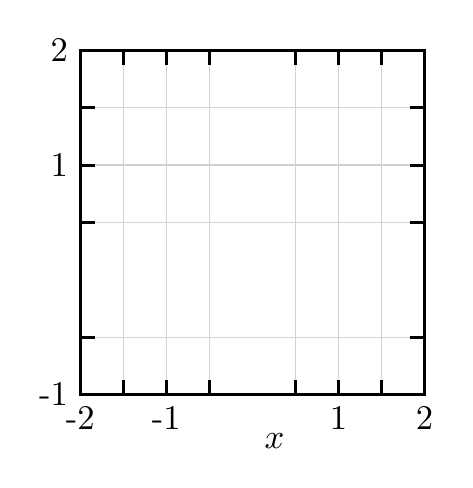
\begin{tikzpicture}[scale=1.25]
          \begin{axis}[
        %    axis y line = left,
            axis  line style= {line width = 1pt},
            xlabel={$x$},
            xtick       = {-2,-1.5,-1,-.5, .5,1,1.5,2},
            xticklabels = {-2,,-1,,,1,,2},
            ytick       = {-1,-.5,.5,1,1.5,2},
             yticklabels = {-1,,,1,,2},
             major tick style = {black, thick},
            xlabel style={anchor=west},
            ylabel style={anchor=south},
            samples     = 160,
            domain      = -1.25:1.15,
            xmin = -2, xmax = 2,
            ymin = -1, ymax = 2,
            grid=both, grid style={gray!35},
            width=2in, height=2.in
          ]
          %\addplot[domain=-2:2, blue, ultra thick, -] {abs(x)};
        \end{axis}
    \end{tikzpicture}
    }{       
     \begin{enumerate}
        \item[(b)] Compute $\ds \int_{-1}^1 \left(f(x) + 1\right) dx.$ {\em Hint:} There are at least two reasonable approaches to this question. One approach might be to sketch the graph of $y=f(x)+1$.  An alternative approach might be to use the linearity property of definite integrals. There might be other reasonable approaches as well,
        \end{enumerate}
        }
        
           \mpageT{.4}{.6}{
                   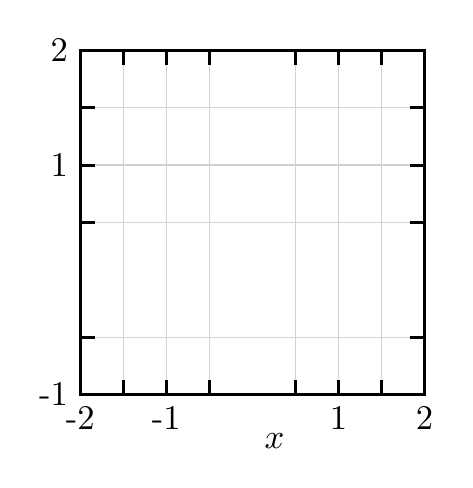
\begin{tikzpicture}[scale=1.25]
          \begin{axis}[
        %    axis y line = left,
            axis  line style= {line width = 1pt},
            xlabel={$x$},
            xtick       = {-2,-1.5,-1,-.5, .5,1,1.5,2},
            xticklabels = {-2,,-1,,,1,,2},
            ytick       = {-1,-.5,.5,1,1.5,2},
             yticklabels = {-1,,,1,,2},
             major tick style = {black, thick},
            xlabel style={anchor=west},
            ylabel style={anchor=south},
            samples     = 160,
            domain      = -1.25:1.15,
            xmin = -2, xmax = 2,
            ymin = -1, ymax = 2,
            grid=both, grid style={gray!35},
            width=2in, height=2.in
          ]
          %\addplot[domain=-2:2, blue, ultra thick, -] {abs(x)};
        \end{axis}
    \end{tikzpicture}
    }{    
        \begin{enumerate}
        \item[(c)] Compute $\ds \int_{-1}^1 f(x + 1)\;dx.$ {\em Hint:} It will be helpful to sketch the graph of $y=f(x+1)$.
    \end{enumerate}
    }
\end{enumerate}
\newpage
\section{Properties of the Definite Integral}
\begin{enumerate}
    \item Consider the following graph of $f(x).$
\begin{center}
      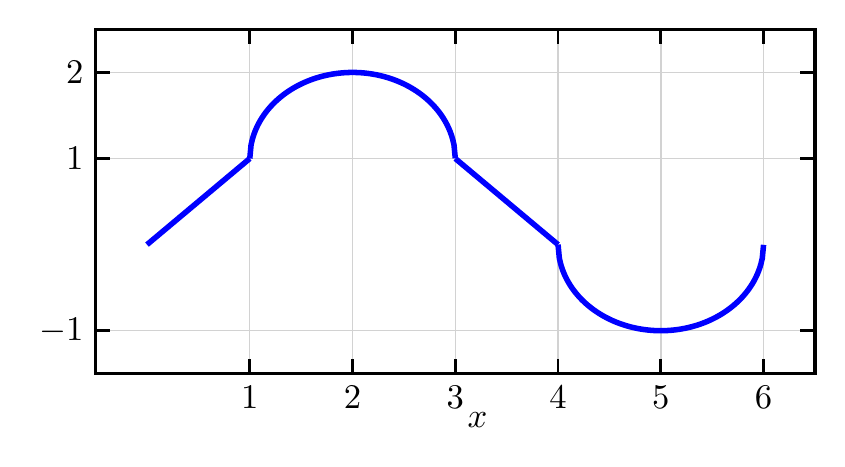
\begin{tikzpicture}[scale=1.25]
          \begin{axis}[
        %    axis y line = left,
            axis  line style= {line width = 1pt},
            xlabel={$x$},
            xtick       = {1,2,3,4,5,6},
            %xticklabels = {-2,,-1,,,1,,2},
            ytick       = {-1,1,2},
           %  yticklabels = {-1,,,1,,2},
             major tick style = {black, thick},
            xlabel style={anchor=west},
            ylabel style={anchor=south},
            samples     = 160,
            domain      = -1.25:1.15,
            xmin = -.5, xmax = 6.5,
            ymin = -1.5, ymax = 2.5,
            grid=both, grid style={gray!35},
            width=3.5in, height=2.in
          ]
          \addplot[domain=0:1, blue, ultra thick, -] {x};
          \addplot[domain=1:3, blue, ultra thick, -] {sqrt(1-(x-2)^2)+1};
		\addplot[domain=3:4, blue, ultra thick, -] {4-x};
 		\addplot[domain=4:6, blue, ultra thick, -] {-sqrt(1-(x-5)^2)};
        \end{axis}
    \end{tikzpicture}
\end{center}
    \begin{enumerate}
        \item[(a)] Compute $\ds \int_0^6 f(x) \;dx$ exactly.
        \item[(b)] Compute $\ds \int_2^4 f(x) \;dx$ exactly.
        \item[(c)] Challenge question: Compute $\ds \int_0^6 |f(x)| dx.$
    \end{enumerate}

    \newpage
    \item Given the knowledge that 
    $$\int_1^5 f(x)dx = 10, \int_1^{10} f(x)dx = -1 \text{ and } \int_{-1}^1 f(x)\;dx= 8$$
    compute:
    \begin{enumerate}
        \item $\ds \int_5^{10} f(x)dx$
        \item $\ds \int_{-1}^{10} f(x)dx$
        \item $\ds \int_{-1}^5 f(x) dx$
        \item $\ds \int_{10}^1 f(x) dx$
    \end{enumerate}
\end{enumerate}
\newpage
 \section{Optimization} 
 \begin{enumerate}
     \item We want to construct a cylindrical can with a bottom but no top that will have a volume of 30 $cm^3$. What is the minimum surface area that such a cylinder can have? \\\\Note that the volume of a cylinder of height $h$ is $\ds V=\pi r^2\dot h$ and the surface area  is $SA=2\pi r\cdot h$
     \newpage
     \item We want to find two positive numbers, $a$ and $b,$ whose product is $250,$ and which minimizes $F=a + 10b.$
 \end{enumerate}
\end{document}